\documentclass[degree=bachelor]{hustthesis-en}
% \usepackage{lua-visual-debug}

\title{An Example of Using hustthesis \LaTeX{} Template}
\author{Xu Cheng}
\major{Electronic and Information Engineering}
\supervisor{Ass. Prof. Xiaojun Hei}
\date{2013}{6}{1}

\abstract{
    This is a \LaTeX{} template example file. This template is used in written thesis for Huazhong Univ. of Sci. \& Tech.

    This template is published under LGPL 2.1 License.
}

\keywords{\LaTeX{}, Huazhong Univ. of Sci. \& Tech., Thesis, Template}

\begin{document}

\frontmatter
\maketitle
\makeabstract
\tableofcontents
\mainmatter

\chapter{Simple Test}

\section{Level 1}
\subsection{Level 2}
\subsubsection{Level 3}
Content

\section{Font}

Normal \textbf{Bold} \emph{Italic} \textsf{Sans}

The quick brown fox jumps over the lazy dog.

\section{Equation}

Single equation, see Equation \ref{eq:1}.
\begin{equation}
  E = mc^2 \label{eq:1}
\end{equation}

Multi-equations, see Equation \ref{eq:2} and \ref{eq:3}.

\begin{subequations}
\begin{equation}
  F = ma \label{eq:2}
\end{equation}
\begin{equation}
  c^2 = a^2 + b^2 \label{eq:3}
\end{equation}
\end{subequations}

\section{List Environment}

\begin{enumerate}
    \item Level 1
    \item Level 1
    \begin{enumerate}
        \item Level 2
        \item Level 2
        \begin{enumerate}
            \item Level 3
            \item Level 3
        \end{enumerate}
    \end{enumerate}
\end{enumerate}

\begin{description}
    \item[Discription]  Content
\end{description}

\chapter{Other Test}

\section{Code Highlight}

\begin{lstlisting}[language=python]
import os

def main():
    '''
    doc here
    '''
    print 'hello, world' # Abc
\end{lstlisting}

\section{Theorem}

\begin{definition}
This is a definition.
\end{definition}
\begin{proposition}
This is a proposition.
\end{proposition}
\begin{axiom}
This is an axiom.
\end{axiom}
\begin{lemma}
This is a lemma.
\end{lemma}
\begin{theorem}
This is a theorem.
\end{theorem}
\begin{proof}
This is a proof.
\end{proof}

\section{Algorithm}

\begin{algorithm}[H]
\SetAlgoLined
\KwData{this text}
\KwResult{how to write algorithm with \LaTeX2e }
initialization\;
\While{not at end of this document}{
read current\;
\eIf{understand}{
go to next section\;
current section becomes this one\;
}{
go back to the beginning of current section\;
}
}
\caption{How to write algorithms}
\end{algorithm}

\section{Table}
See Table~\ref{tab:1}.

\begin{table}[ht]
\centering
\caption{A table}\label{tab:1}
\begin{tabular}{|c|c|}
\hline
a & b \\
\hline
c & d \\
\hline
\end{tabular}
\end{table}

\section{Figure}
See Figure~\ref{fig:1}.Figure supports format in eps, png, pdf and so on.

\begin{figure}[hb]
\centering
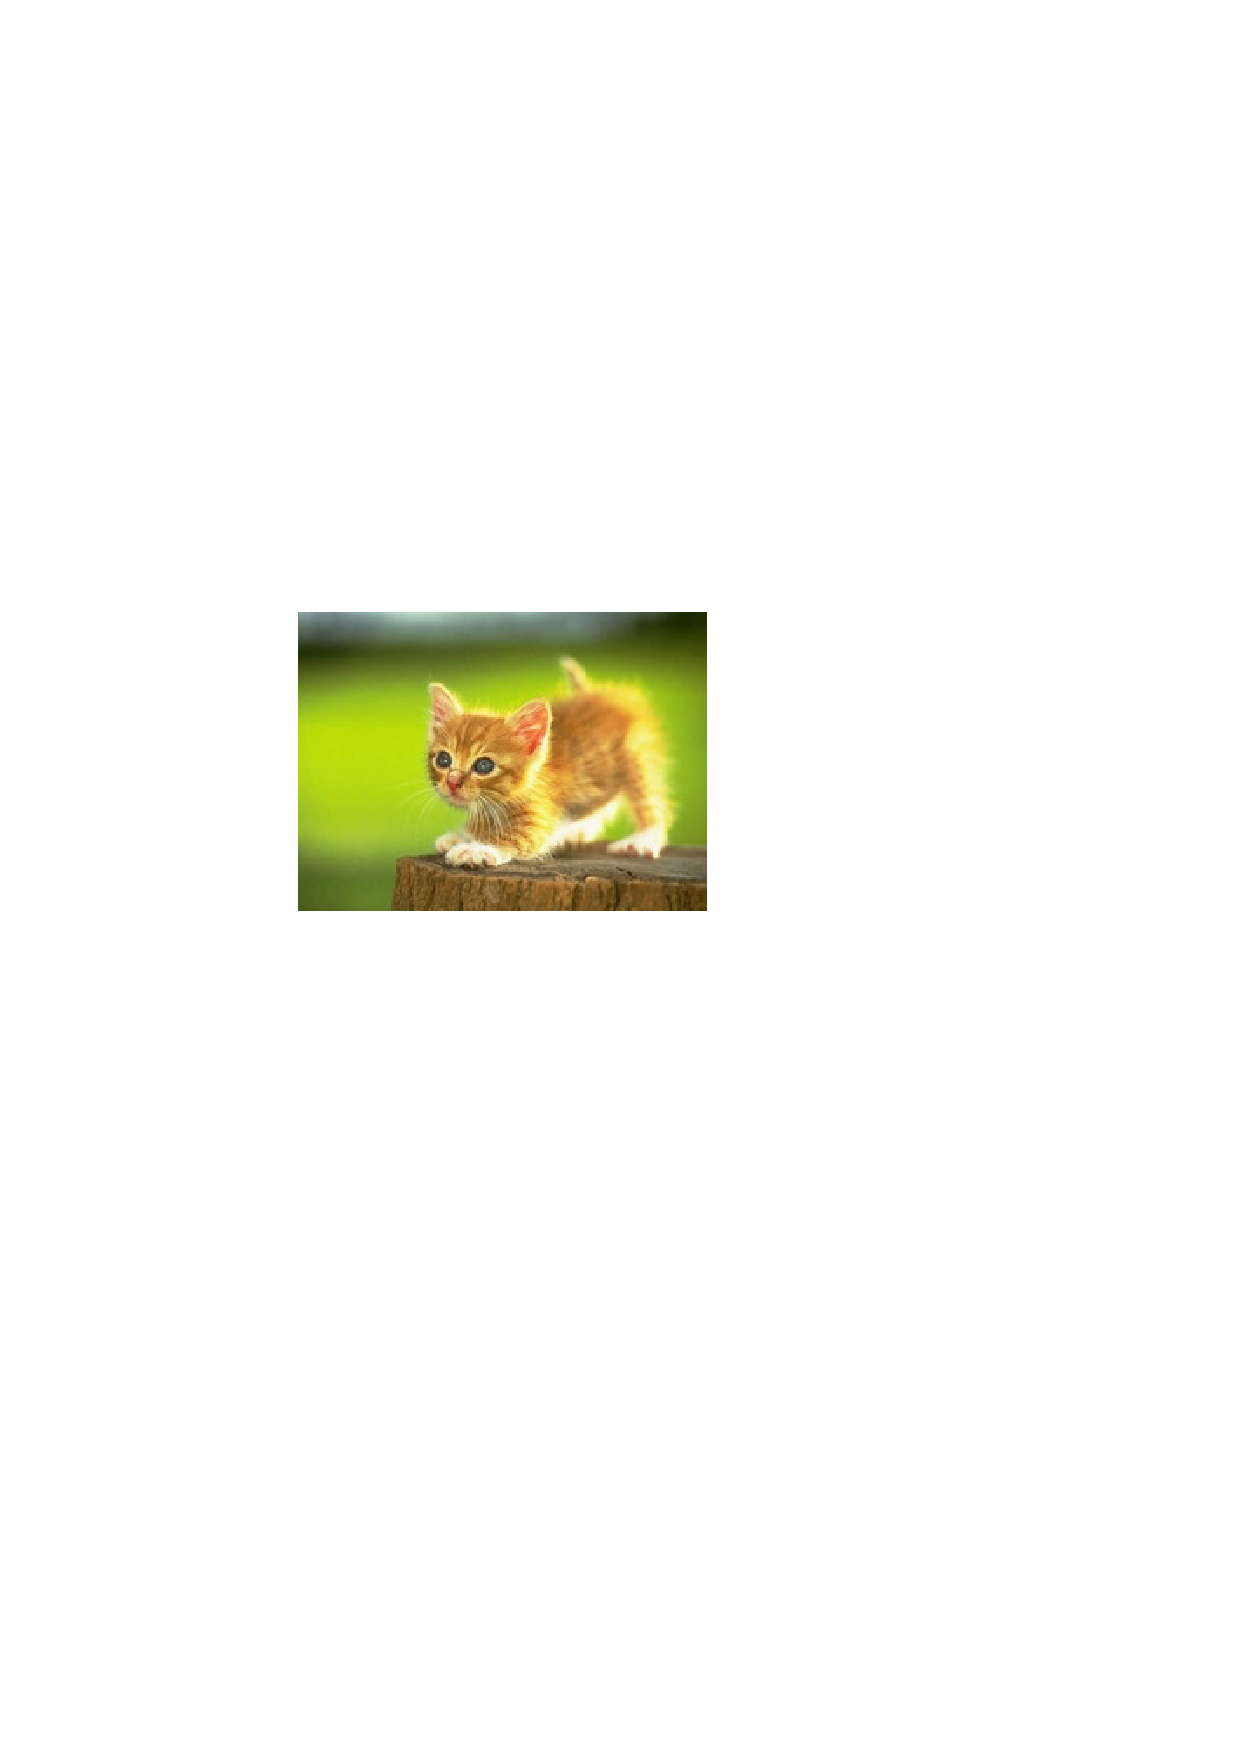
\includegraphics[width=.8\textwidth]{fig-example.pdf}
\caption{A figure}\label{fig:1}
\end{figure}

\section{Bibliography}
Cite one bib\cite{knuth}, cite two\cite{TEXGURU99,knuth}.

\backmatter

\begin{ack}
Acknowledge
\end{ack}

\bibliography{ref-example}

\appendix

\listoffigures
\listoftables

\begin{publications}
    \item Thesis 1
    \item Thesis 2
\end{publications}

\chapter{This is an appendix}
Content.

\end{document}